\section{Tabela assíncrona (JTable)}

Nesta seção veremos como implementar uma tabela \texttt{assíncrona}
(\texttt{JTable}) usando o \texttt{MDArte}. Para tal, vamos considerar como
ponto de partida o modelo do caso de uso \texttt{Consulta Estudante} conforme as
alterações feitas no tópico anterior. Certifique-se de ter removido o
estereótipo \texttt{«Manageable»} da classe \texttt{Estudante} no diagrama de
classes que descreve a \texttt{Camada de domínio}, a fim de evitar que o
\texttt{CRUD} seja re-gerado, sobrescrevendo assim as alterações que faremos.

Veremos agora, por subseções, algumas das funcionalidades disponíveis na tabela
assíncrona.

\subsection{Implementando uma tabela simples}

Para implementar uma tabela assíncrona, precisamos primeiramente abrir o modelo
do caso de uso \texttt{Consulta Estudante}, abriremos então a especificação da
\texttt{transition} que sai da \texttt{action} \texttt{ConsultandoEstudante}
para \texttt{Front End View} \texttt{'ResultadoConsulta'}, clicar no botão
\texttt{edit} no \texttt{fieldset} \texttt{trigger}, iremos então na aba
\texttt{parameters}, na janela \texttt{signal event specification}, aberta
automaticamente. Daremos então um duplo clique no nome do parâmetro
(\texttt{estudantes}), que representa a tabela que será mostrada na view.
Selecionaremos a aba \texttt{tagged values} selecione o \texttt{tagged value}
\texttt{@andromda.presentation.web.view.field.table.type} e clique no botão
\texttt{create value}. Selecione então a opção \texttt{jtable}, como na
imagem \ref{table_type_jtable}.

\begin{figure}[H]
	\centering
	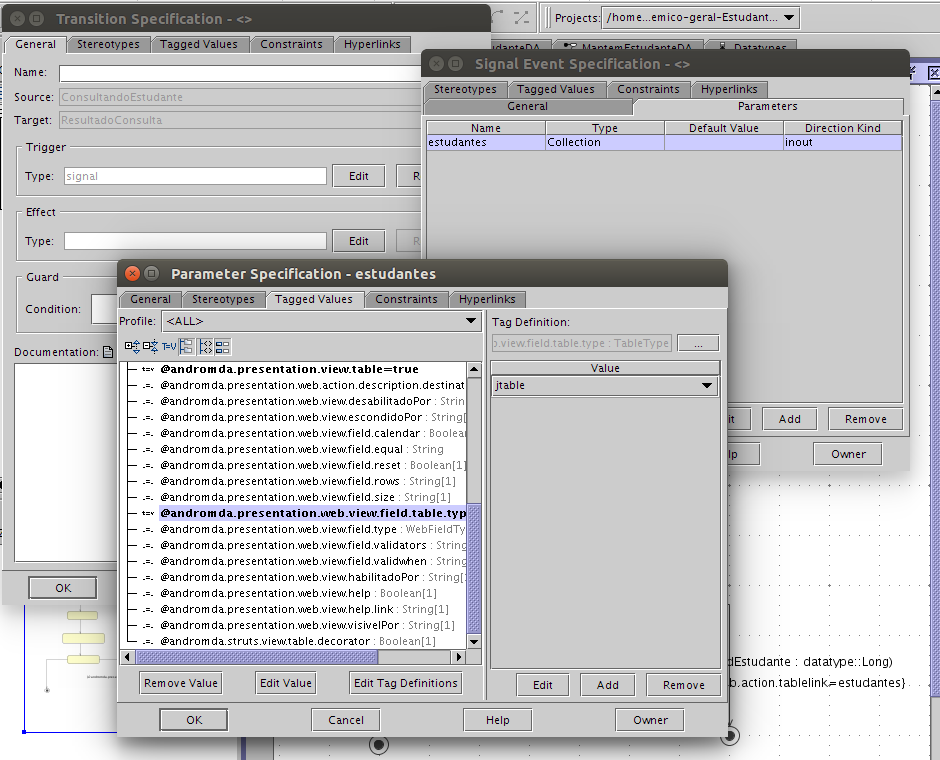
\includegraphics[width=350pt,height=300pt]{files/imgs/tutorial-mdarte-0030.png}
	\caption{Mudando tipo da tabela para 'jtable'.}
	\label{table_type_jtable}
\end{figure}

Agora executaremos o seguinte comando no terminal na raiz do projeto:

\begin{lstlisting}[language=bash, frame=single, breaklines=true]
maven mda -Dprojeto=sistemaacademico-geral-Estudante
\end{lstlisting}

Feito isto, o MDArte já terá gerado toda a estrutura necessária pela recepção e
tratamento das requisições assíncronas da tabela, restando ao desenvolvedor
implementar somente dois métodos: um para indicar o numero total de elementos a
serem exibidos na tabela, usado para fazer a paginação da mesma, e outro para
retornar a coleção de objetos a serem exibidos na página atual da tabela.

A assinatura do método para o carregamento da tabela segue o seguinte padrão:

\begin{lstlisting}[language=java, frame=single, breaklines=true]
protected Collection load[nome-da-view][nome-da-tabela]Table(PaginationStrategy
paginacao, String propriedade, Boolean desc, ViewContainer container)
\end{lstlisting}

A assinatura do método que retorna o total de elementos na tabela segue o
seguinte padrão:

\begin{lstlisting}[language=java, frame=single, breaklines=true]
protected Integer get[nome-da-view][nome-da-tabela]TableLength(PaginationStrategy
paginacao, String propriedade, Boolean desc, ViewContainer
container) throws Exception
\end{lstlisting}

Também será necessário alterar o método \texttt{carregaDados} do
\texttt{ControllerImpl} para disponibilizar as informações preenchidas na
\texttt{PreenchaCampos} para serem usadas pela tabela disponível na
\texttt{view} \texttt{ResultadoConsulta}.

Abaixo o exemplo de implementação para a tabela \texttt{estudantes} da
\texttt{view ResultadoConsulta} no caso de uso \texttt{Consulta Estudante}.

\lstinputlisting[language=java, frame=single, breaklines=true] {files/java/JTableSimples.java}

Não se esqueça de fazer os \texttt{imports} necessários de acordo com as
alterações feitas. Se o seu \texttt{.classpath} estiver corretamente
configurado, você pode usar o atalho \texttt{Ctrl + Shift + O}, do eclipse, que
importará automaticamente todas as classes que estão faltando.

Agora, compilaremos e daremos deploy do código da aplicação, com o seguinte
comando:

\begin{lstlisting}[language=bash, frame=single, breaklines=true]
maven compile deploy
\end{lstlisting}

Abriremos agora a view \texttt{PreenchaCampos} e digitaremos um valor para
filtragem dos dados da entidade \texttt{Estudante}. Como na imagem
\ref{preencha_campos_tabela_async_simples}.

\begin{figure}[H]
	\centering
	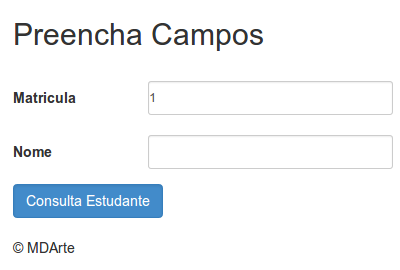
\includegraphics[width=260pt,height=180pt]{files/imgs/tutorial-mdarte-0031.png}
	\caption{Filtrando dados da tabela assíncrona de Estudantes.}
	\label{preencha_campos_tabela_async_simples}
\end{figure}

Na imagem \ref{resultado_consulta_tabela_async_simples}, podemos ver a tabela
carregada com os dados resultantes da filtragens.

\begin{figure}[H]
	\centering
	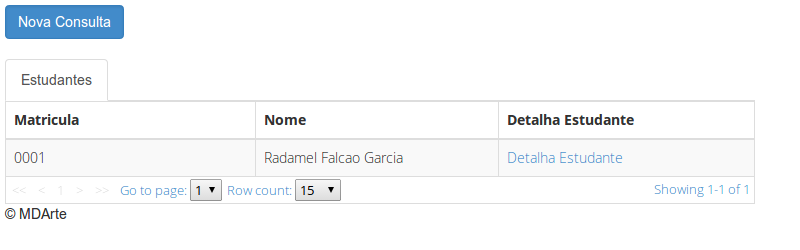
\includegraphics[width=460pt,height=200pt]{files/imgs/tutorial-mdarte-0032.png}
	\caption{Filtragem dos dados da tabela assíncrona de Estudantes.}
	\label{resultado_consulta_tabela_async_simples}
\end{figure}

Note que o funcionamento da tabela se dá por requisições assíncronas
ao servidor, acabando com a necessidade de recarregar a página para alterar seus
dados. 

O \texttt{MDArte} já dá suporte a diversos tipos de chamadas assíncronas que se
possa querer fazer fazer com a tabela, no entanto, caso haja a necessidade de
mais informações sobre o funcionamento da mesma, a documentação pode ser
acessada \href{http://www.jtable.org/Home/Documents}{aqui}.

\subsection{Implementando filtragem assíncrona da tabela}
Nesta seção veremos como criar uma action ajax que reflita nos dados exibidos
por uma tabela ajax. A título de exemplo, faremos uma tela com um formulário e
um botão que, uma vez clicado, recarregará a tabela filtrando-a de acordo com os
dados do formulário. Tomaremos como base a tabela criada no exemplo de criação
de tabelas.

O modelo portanto começará assim:

\begin{figure}[H]
	\centering
	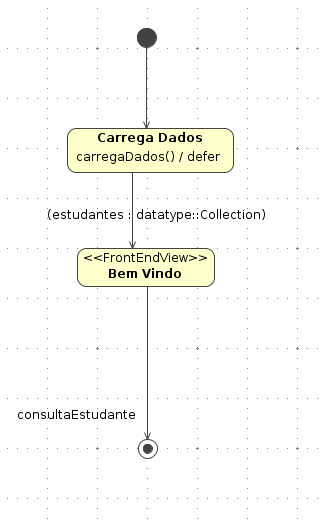
\includegraphics[width=180pt,height=260pt]{files/imgs/tutorial-mdarte-0040.png}
	\caption{Modelagem da filtragem assíncrona da tabela.}
	\label{modelando_filtragem_assincrona}
\end{figure}

Modelaremos então uma \texttt{transition} saindo da \texttt{FrontEndView} que
contém a nossa tabela e retornando para a mesma \texttt{view}, que será
interpretada pelo \texttt{MDArte} como uma ação assíncrona na \texttt{view}.
Abriremos então sua especificação e iremos na aba \texttt{tagged values} e
selecionaremos o \texttt{tagged value}
\texttt{@andromda.presentation.web.action.async.table} e daremos a ele o valor
\texttt{[nome-da-tabela]} (\texttt{estudantes}, nesse caso), esse \texttt{tagged
value} indica qual tabela será afetada pela ação assíncrona, nos permitindo ter
mais de uma de tabela assíncrona na mesma tela, tendo \texttt{actions} que
afetem somente uma tabela sem afetar a outra. Iremos então na aba
\texttt{general} e clicaremos no botão \texttt{edit} no \texttt{fieldset}
\texttt{'trigger'}, daremos o nome que desejarmos o \texttt{trigger} criado, no
exemplo fo idado o nome de \texttt{“filtrar”}, e selecionaremos seu tipo como
\texttt{signal}. Iremos então na aba \texttt{parameters}, ainda na especificação
do \texttt{trigger} e criaremos os parâmetros necessários para o processamento
da requisição, neste exemplo colocaremos só os parâmetros \texttt{matrícula} e
\texttt{nome}, a título de ilustração, e definiremos seus tipos como
\texttt{String}.

O modelo ficará assim:
\begin{figure}[H]
	\centering
	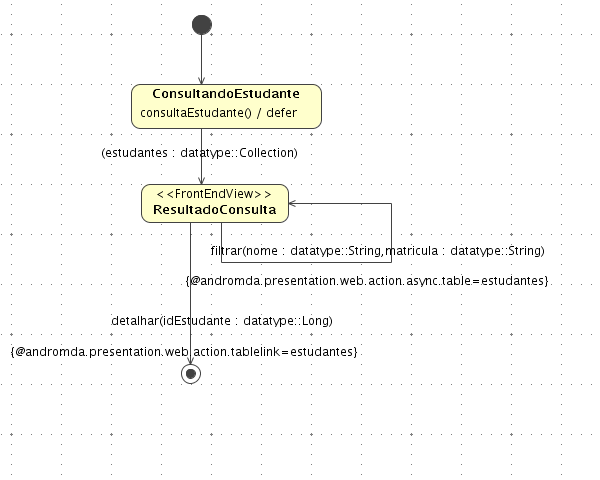
\includegraphics[width=340pt,height=300pt]{files/imgs/tutorial-mdarte-0036.png}
	\caption{Modelagem da filtragem assíncrona da tabela.}
	\label{modelando_filtragem_assincrona}
\end{figure}

Executaremos agora o seguinte comando para validar o modelo e regerar o
sistema:
\begin{lstlisting}[language=bash, frame=single, breaklines=true]
maven mda -Dprojeto=sistemaacademico-geral-Estudante
\end{lstlisting}

Agora adaptaremos, no \texttt{ControleImpl}, os métodos responsáveis pelo
carregamento da tabela, com a assinatura \texttt{public final Collection
load[nome-da-view][nome-da-tabela]Table}, e pelo retorno do número máximo de
elementos na mesma, com a assinatura \texttt{public final Integer
get[nome-da-view][nome-da-tabela]TableLength}, a fim de implementarmos o filtro.
Cada parâmetro da \texttt{trigger} pertencente à \texttt{transition} modelada
será adicionado, em ordem, à lista de parâmetros de cada método, logo antes do
parâmetro \texttt{ViewContainer container}. De acordo com o nosso exemplo, o
código ficará assim:
\lstinputlisting[language=java, frame=single, breaklines=true]{files/java/JTableFiltro.java}

Executaremos agora o seguinte comando para compilar e dar \texttt{deploy} no
sistema:
\begin{lstlisting}[language=bash, frame=single, breaklines=true]
maven compile deploy
\end{lstlisting}

Restartando o servidor e abrindo o caso de uso \texttt{Consulta Estudante},
veremos o resultado do que fizemos:
\begin{figure}[H]
	\centering
	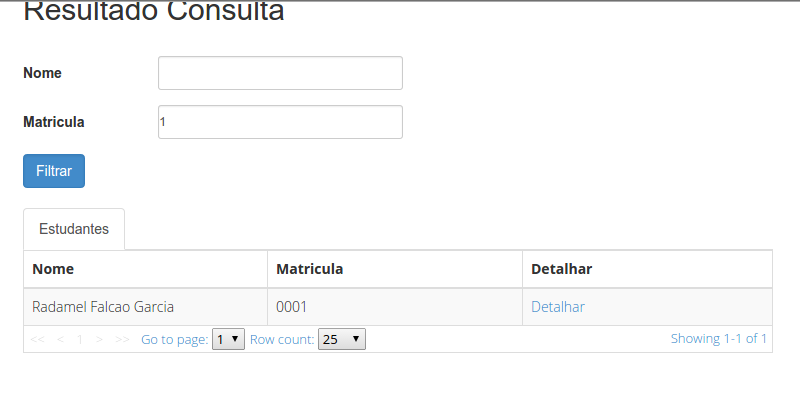
\includegraphics[width=340pt,height=300pt]{files/imgs/tutorial-mdarte-0042.png}
	\caption{Modelagem da filtragem assíncrona da tabela.}
	\label{modelando_filtragem_assincrona}
\end{figure}
